%%%%%%%%%%%%%%%%%%%%%%%%%%%%%%%%%%%%%%%%%%%%%%%%%%%%%%%%%%%%%%%%%%%%%%%%%%%%%%%%
% CS 598 FTS Final Report -- Removing the Sister-Replica Assumption from Pesto
%%%%%%%%%%%%%%%%%%%%%%%%%%%%%%%%%%%%%%%%%%%%%%%%%%%%%%%%%%%%%%%%%%%%%%%%%%%%%%%%

\documentclass[letterpaper,twocolumn,10pt]{article}
\usepackage{usenix2019_v3}

\usepackage{tikz}
\usetikzlibrary{positioning,shapes.geometric,arrows.meta,fit,calc,backgrounds}
\usepackage{amsmath}
\usepackage{booktabs}
\usepackage{graphicx}

%-------------------------------------------------------------------------------
\begin{document}
%-------------------------------------------------------------------------------

\date{}

\title{\Large \bf Removing the Sister-Replica Assumption \\
       from a BFT SQL Database}

\author{
{\rm Jiatong Li}\\
University of Illinois Urbana-Champaign\\
\texttt{jl180@illinois.edu}
\and
{\rm Otto Piramuthu}\\
University of Illinois Urbana-Champaign\\
\texttt{obp2@illinois.edu}
}

\maketitle

%-------------------------------------------------------------------------------
\begin{abstract}
%-------------------------------------------------------------------------------
Pesto~\cite{pesto25}, the SOSP'25 Byzantine-fault-tolerant SQL database,
performs cross-shard coordination under a strong assumption: every
trust authority operates a replica in \emph{every} shard, so that
intra-shard quorum decisions can be implicitly trusted by sibling
replicas in other shards. This ``sister-replica'' assumption is
unrealistic for federated, multi-organization deployments.

We remove the assumption by introducing two new artifacts:
(i)~\emph{Shard Membership Certificates}, which cryptographically attest
to a shard's replica set; and (ii)~\emph{Cross-Shard Snapshot
Certificates v3-STRICT (SS-CERT v3-STRICT)}, which bind a content
digest to a $2f{+}1$ Ed25519-signed quorum decision and survive
cross-shard verification. We implement these on top of the Pesto
artifact and evaluate on a 38-node CloudLab cluster spanning $f{=}1$,
$f{=}2$, and $f{=}3$.

Across $\approx{250}$ experiments and roughly $1.05$~million v3-STRICT
verifications under both honest and Byzantine workloads (omission and
twin-equivocation faults), we observe zero spurious cert accepts.
Removing the sister-replica assumption costs only $1{-}5\%$ throughput
at the same fault budget. A surprising side effect of our content-bound
quorum is improved saturation behavior: at $\mathrm{NC}\geq 18$ our
extension delivers $1.5\times$ to $3.85\times$ the throughput of
original Pesto.
\end{abstract}


%-------------------------------------------------------------------------------
\section{Introduction}
%-------------------------------------------------------------------------------

Modern BFT databases~\cite{basil21,pesto25} achieve impressive
throughput by sharding state across replicated groups and by exploiting
optimistic fast paths for cross-shard transactions. However, sharded
designs typically require some cross-shard trust mechanism so that one
shard can act on a fact established at another shard.

Pesto solves this by assuming that every trust authority runs a replica
in every shard (Appendix~B.10 of~\cite{pesto25}). With sister replicas,
shard~A's replica~$i$ is operated by the same organization as
shard~B's replica~$i$, and so its commit decision can be trusted at
shard~B without explicit cryptographic proof. This is convenient but
unrealistic: in a federated deployment (e.g., a consortium of banks
where each member runs only its local shard), a regulator's shard
should not have to trust a competitor's intra-shard quorum decision
without a cryptographic certificate.

\paragraph{Our contribution.} This project removes the sister-replica
assumption from Pesto without sacrificing safety or peak throughput.
We add:
\begin{itemize}\setlength{\itemsep}{2pt}
\item \textbf{Shard Membership Certificates} that attest to a shard's
      replica set (group ID, fault budget $f$, replica IDs, public
      keys, BLAKE3 digest);
\item \textbf{SS-CERT v3-STRICT}: cross-shard snapshot certificates
      whose digest is content-bound to the query result hash, requiring
      $2f{+}1$ distinct Ed25519 signatures all attesting to the same
      content;
\item \textbf{Heterogeneous-quorum runtime}: per-shard $n$ and $f$ and
      per-group quorum bounds throughout the protocol stack.
\end{itemize}

We implement on the Pesto artifact (an extension of
Basil~\cite{basil21}) and evaluate on $38$ CloudLab~\cite{cloudlab}
nodes. We validate both safety (Adya G0/G1/G2 cycles via
Elle~\cite{elle}, cross-shard atomicity, $2f{+}1$ cert integrity) and
performance (sister-replica vs.\ heterogeneous deployment, saturation
curves, WAN tolerance, and a head-to-head comparison against the
unmodified Pesto binary).

The most striking finding is a \emph{crossover}: at low client load
($\mathrm{NC}=6$) original Pesto is $58\%$ faster than our extension
(the cost of the extra crypto), but at moderate load
($\mathrm{NC}\geq 12$) our extension matches or surpasses original
Pesto, and at high load ($\mathrm{NC}=24$) our extension delivers
$3.85\times$ the throughput because the v3-STRICT histogram filter
incidentally smooths cross-replica timing variance.


%-------------------------------------------------------------------------------
\section{Background and Motivation}
%-------------------------------------------------------------------------------

\paragraph{Pesto in 30 seconds.} Pesto is a sharded BFT database where
each shard runs a Basil-style two-phase commit with $n=5f+1$ replicas
and tolerates up to $f$ Byzantine replicas per shard. A cross-shard
transaction's client coordinates a 2PC across the involved shards; each
shard locally produces a snapshot certificate (\textbf{SS-CERT}) that
its sibling shards consume to advance the global commit decision.

\paragraph{The sister-replica assumption.} Pesto's SS-CERT does not
itself contain a $2f{+}1$ signature quorum. Instead, the receiving
shard implicitly trusts the sending shard because the same trust
authority operates one replica in each shard. The cert effectively
contains \emph{one} signature from one's own sister, which is taken as
the shard's collective decision. This assumption is what we remove.

\paragraph{Why it matters.} The sister-replica assumption forces
every participating organization to operate a replica in every shard.
For a 5-shard system shared by 11 organizations, this is $55$ replica
processes per organization. It also leaks operational risk: if one
organization compromises its $i$-th replica in every shard
simultaneously, the global trust model collapses. In a
multi-organization deployment, one expects to be able to participate
in only the shards one cares about.

\paragraph{What changes when we remove it.} Without sister replicas,
shard~B's protocol path that consumed shard~A's SS-CERT must now
verify that the cert was produced by a $2f{+}1$ Byzantine quorum of
shard~A's replicas, using only public keys derivable from shard~A's
membership certificate. This requires reworking the certificate format,
the per-replica vote-signing path, the client-side cert-assembly path
(it must collect $2f{+}1$ matching votes), and the receiving shard's
verifier. We also need a way to expose shard~A's membership to
shard~B in the first place, which is the role of the membership cert.


%-------------------------------------------------------------------------------
\section{Design}
%-------------------------------------------------------------------------------


%---------------------------------------------------------------
% Architecture figure (TikZ)
%---------------------------------------------------------------
\begin{figure*}[t]
\centering
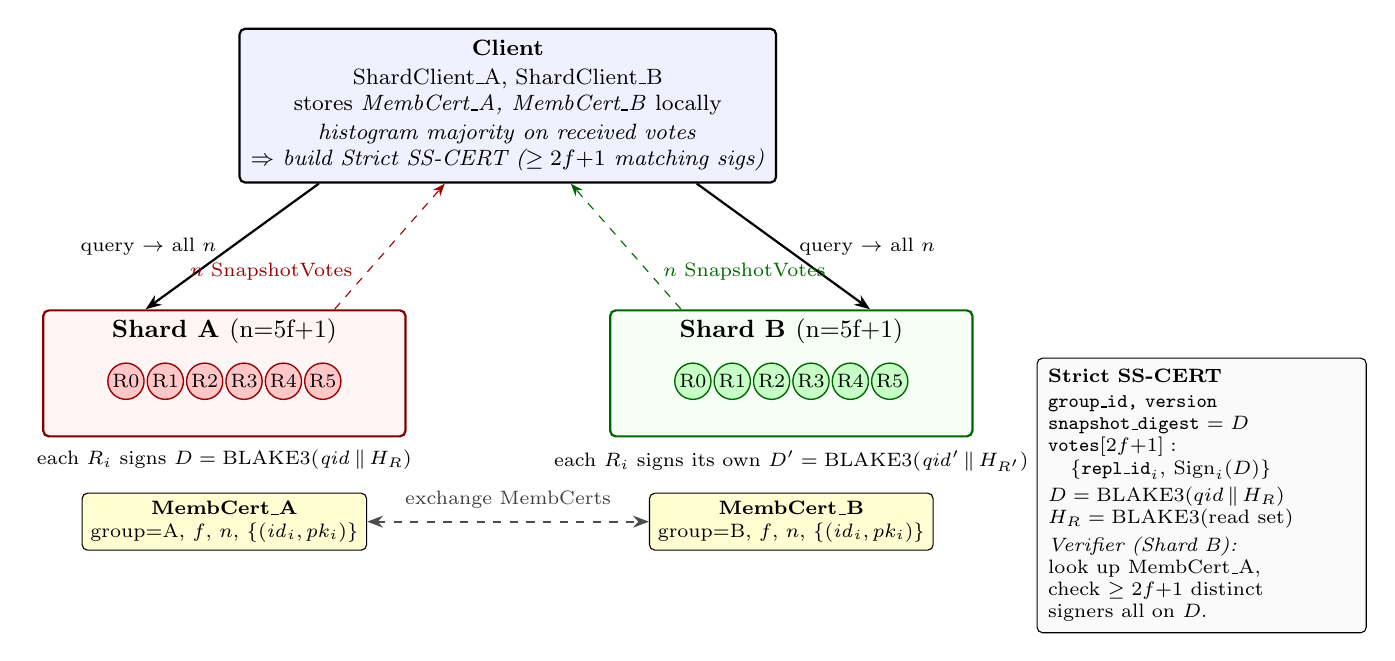
\begin{tikzpicture}[
  font=\footnotesize,
  shard/.style    = {draw, rounded corners=2pt, thick, minimum width=4.6cm,
                     minimum height=1.6cm, align=center, inner sep=4pt},
  replica/.style  = {draw, circle, minimum size=0.46cm, inner sep=0pt,
                     font=\scriptsize, line width=0.5pt},
  cert/.style     = {draw, fill=yellow!18, rounded corners=2pt,
                     minimum width=2.6cm, align=center, font=\scriptsize,
                     inner sep=3pt},
  client/.style   = {draw, rounded corners=2pt, thick, fill=blue!6,
                     minimum width=6.4cm, minimum height=1.4cm,
                     align=center, inner sep=4pt},
  inset/.style    = {draw, fill=gray!4, rounded corners=2pt,
                     align=left, font=\scriptsize, inner sep=4pt},
  arrow/.style    = {-{Stealth[length=2mm]}, thick},
  thinarrow/.style= {-{Stealth[length=1.6mm]}, thin},
  dasharrow/.style= {{Stealth[length=2mm]}-{Stealth[length=2mm]}, thick,
                     dashed},
  >=Stealth,
]

% ===== Client (top center) =====
\node[client] (client) at (0, 4.4) {%
  \textbf{Client} \\[1pt]
  ShardClient\_A, ShardClient\_B \\
  stores \textit{MembCert\_A, MembCert\_B} locally \\[1pt]
  \emph{histogram majority on received votes} \\
  \emph{$\Rightarrow$ build Strict SS-CERT ($\geq 2f{+}1$ matching sigs)}
};

% ===== Shard A (bottom left) =====
\node[shard, fill=red!4, draw=red!50!black] (shardA) at (-3.6, 1.0) {};
\node[anchor=north, font=\small\bfseries] at (shardA.north)
      {Shard A \normalfont(n=5f+1)};
\foreach \i in {0,...,5} {
  \node[replica, fill=red!22, draw=red!60!black]
        at ($(shardA.center) + (-1.25 + 0.5*\i, -0.10)$) {R\i};
}
\node[anchor=north, font=\scriptsize] at ($(shardA.south) + (0,-0.04)$)
      {each $R_i$ signs $D=\mathrm{BLAKE3}(\mathit{qid}\,\|\,H_R)$};
\node[cert, anchor=north] (certA) at ($(shardA.south) + (0,-0.7)$)
      {\textbf{MembCert\_A} \\ group=A, $f$, $n$, $\{(\mathit{id}_i, pk_i)\}$};

% ===== Shard B (bottom right) =====
\node[shard, fill=green!4, draw=green!40!black] (shardB) at (3.6, 1.0) {};
\node[anchor=north, font=\small\bfseries] at (shardB.north)
      {Shard B \normalfont(n=5f+1)};
\foreach \i in {0,...,5} {
  \node[replica, fill=green!22, draw=green!40!black]
        at ($(shardB.center) + (-1.25 + 0.5*\i, -0.10)$) {R\i};
}
\node[anchor=north, font=\scriptsize] at ($(shardB.south) + (0,-0.04)$)
      {each $R_i$ signs its own $D'=\mathrm{BLAKE3}(\mathit{qid}'\,\|\,H_{R'})$};
\node[cert, anchor=north] (certB) at ($(shardB.south) + (0,-0.7)$)
      {\textbf{MembCert\_B} \\ group=B, $f$, $n$, $\{(\mathit{id}_i, pk_i)\}$};

% ===== Query (down) arrows: anchored INSIDE client/shard frames =====
% Client horizontal extent: roughly -3.2 .. +3.2.  Use -2.4 and +2.4 so the
% arrow tail clearly sits on the client's bottom edge.
\draw[arrow] ($(client.south) + (-2.4,0)$) -- ($(shardA.north) + (-1.0,0)$)
   node[midway, left=2pt, font=\scriptsize] {query $\to$ all $n$};
\draw[arrow] ($(client.south) + ( 2.4,0)$) -- ($(shardB.north) + ( 1.0,0)$)
   node[midway, right=2pt, font=\scriptsize] {query $\to$ all $n$};

% ===== Vote return arrows: parallel, offset, dashed.
%   Labels placed at pos=0.3 (bottom of the V where arrows are widest apart)
%   and anchored OUTWARD (red label extends left, green extends right) so the
%   two labels cannot overlap.  "Sign_i(D)" is omitted from these labels since
%   each shard's bottom caption already states what is signed.
\draw[thinarrow, dashed, draw=red!60!black]
   ($(shardA.north) + (1.4,0)$) -- ($(client.south) + (-0.8,0)$)
   node[pos=0.3, left=2pt, font=\scriptsize, text=red!60!black]
        {$n$ SnapshotVotes};
\draw[thinarrow, dashed, draw=green!40!black]
   ($(shardB.north) + (-1.4,0)$) -- ($(client.south) + (0.8,0)$)
   node[pos=0.3, right=2pt, font=\scriptsize, text=green!40!black]
        {$n$ SnapshotVotes};

% ===== Bootstrap exchange: short dashed arrow BETWEEN MembCert cards =====
\draw[dasharrow, draw=gray!60!black] (certA.east) -- (certB.west)
   node[midway, above=1pt, font=\scriptsize, text=gray!50!black]
        {exchange MembCerts};

% NOTE: the "client -> Shard B forwards SS-CERT_A" arrow was removed because
% it crowded the inset and its terminus on shardB.north_east was visually
% ambiguous (looked like it pointed past the shard).  The cross-shard verify
% semantics is conveyed by the inset's Verifier description and the caption.

% ===== Inset: Strict SS-CERT structure, placed under the cross-shard arrow
%   on the far right -- well clear of all other arrows/labels.
\node[inset, anchor=north west, text width=3.9cm]
      at ($(shardB.east) + (0.8, 0.2)$) {%
  \textbf{Strict SS-CERT}\\[1pt]
  \texttt{group\_id, version}\\
  \texttt{snapshot\_digest} $= D$\\
  \texttt{votes}$[2f{+}1]:$\\
  \quad $\{\texttt{repl\_id}_i,\, \mathrm{Sign}_i(D)\}$\\[2pt]
  $D = \mathrm{BLAKE3}(qid \,\|\, H_R)$\\
  $H_R = \mathrm{BLAKE3}(\text{read set})$\\[2pt]
  \emph{Verifier (Shard B):}\\
  look up MembCert\_A,\\
  check $\geq 2f{+}1$ distinct\\
  signers all on $D$.
};

\end{tikzpicture}
\caption{Architecture of cross-shard heterogeneous Pesto with our
\emph{Strict SS-CERT} (called \texttt{SS-CERT v3-STRICT} in the
implementation; ``v3'' is the third iteration in our internal
design history). Each shard runs $n=5f{+}1$ replicas with a
\emph{disjoint} replica set: no sister-replica assumption. Each
shard publishes a \texttt{MembershipCert} that peer shards load at
bootstrap (dashed double arrow between the cert cards). The client
fans the query out to every replica of every involved shard (solid
down arrows); each replica replies with a SnapshotVote signing a
content-bound digest $D$ (dashed up arrows). The client buckets
received votes by $D$ (histogram majority) and constructs a Strict
SS-CERT containing the $2f{+}1$ matching signatures. The cert is
then forwarded to the peer shard, which re-checks every signature
against its locally stored copy of the originating MembershipCert
(see right-hand callout).}
\label{fig:arch}
\end{figure*}

\subsection{Shard membership certificate}

Each shard, at startup, generates a \texttt{ShardMembershipCert}
containing: \texttt{group\_id}, \texttt{version} (monotonic for
membership rotation), $f$ (fault budget), $n$ (replica count), the
list of \texttt{(replica\_id, public\_key)} pairs, and a BLAKE3 digest
over fields 1--5. The cert is exchanged with peer shards out-of-band
(in our prototype, every shard loads every peer's cert on bootstrap;
production would use a control-plane gossip step).

A receiving shard, on seeing an SS-CERT from group~$g$, looks up the
local copy of group~$g$'s membership cert and uses it both to (i)
validate that each signing replica is a member of group~$g$, and (ii)
fetch the public key for verifying each signature.

\subsection{SS-CERT v3-STRICT}

Each replica that processes a cross-shard query computes a content
digest $D = \mathrm{BLAKE3}(\textit{qseq} \,\|\, \textit{qcli} \,\|\,
\textit{qver} \,\|\, \textit{qgrp} \,\|\, H_R)$, where $H_R$ is the
BLAKE3 hash of the query's read set. The replica then signs $D$ with
its Ed25519 private key, returning a \texttt{Snapshot\-Vote} that carries
both the signature and the exact bytes of $D$.

The client harvests votes from \emph{all} replicas (we use
\texttt{--pequin\_query\_messages=query-all} so the query is fanned out
to all $n$ replicas of each shard). It buckets the received votes by
$D$ and selects the bucket of largest size as the \emph{majority
digest}. If the majority bucket has $\geq 2f{+}1$ distinct signers,
the client constructs an SS-CERT v3-STRICT containing those $2f{+}1$
signatures and the agreed-on $D$.

A receiving shard verifies an SS-CERT v3-STRICT by:
\begin{enumerate}\setlength{\itemsep}{2pt}
\item checking the cert's \texttt{group\_id} and
      \texttt{membership\_version} against the locally stored
      membership cert;
\item requiring $\geq 2f{+}1$ distinct \texttt{replica\_id}s, each
      member of group~$g$;
\item verifying every signature using the public key from the
      membership cert.
\end{enumerate}

\paragraph{Why content binding matters.} The earlier v0 cert (Pesto's
original) signed only the query identity, not the result. A Byzantine
sister replica could trivially attach a valid v0 signature to a
fabricated result. v3-STRICT's content binding means that to forge a
cert, an adversary must control $2f{+}1$ replicas \emph{that all
return the same fabricated content}, which is at least as hard as the
underlying BFT safety threshold.

\subsection{Heterogeneous-quorum runtime}

The original Pesto binary hard-codes ``replica $i$ in group~$g$ has
global ID $= g \cdot n + i$,'' which assumes uniform $n$ and the same
replica index space across groups. We replace this with a
\texttt{GlobalReplicaId(g, i)} accessor that uses cumulative offsets,
and add per-group quorum-size accessors (\texttt{QuorumSize(group)},
\texttt{SlowCommitQuorumSize(group)}, etc.). Every protocol site that
previously used the global $n$ and $f$ now passes a group ID. This
unblocks deployments where shards have different replica counts.


%-------------------------------------------------------------------------------
\section{Implementation}
%-------------------------------------------------------------------------------

The implementation lives on the
\texttt{cross-shard-membership} branch of our
fork.\footnote{\url{https://github.com/ljtsparky/Pequin-Artifact}} It
spans $\sim$30 commits to $\sim$15 files in
\texttt{src/store/pequinstore/}. Key components:

\begin{description}\setlength{\itemsep}{2pt}
\item[\texttt{membership.h/cc}] Shard membership cert generator and
      store. Each server generates its own group's cert at boot.
\item[\texttt{server.cc}] Adds \texttt{GenerateSnapshotVote},
      \texttt{VerifyForeignSSCert}, and the v3 self-test that runs at
      startup as a sanity check.
\item[\texttt{querysync-server.cc}] Replaces the v0 sign with the
      content-bound v3 sign in \texttt{SendQueryReply}, and adds the
      twin-replica byzantine mode (XOR-perturb $H_R$ before signing).
\item[\texttt{querysync-client.cc}] Adds the histogram-majority +
      harvest-before-done cert-assembly logic. The cert is built only
      when $\geq 2f{+}1$ votes match on $D$.
\item[\texttt{common.cc}] Adds per-group \texttt{QuorumSize},
      \texttt{IsReplicaInGroupHeterogeneous}, and
      \texttt{VerifySnapshotCert}.
\end{description}

The orchestrator \texttt{run\_byzantine\_experiment.sh} drives all
experiments on CloudLab. It generates \texttt{shard.config} per run,
launches servers and clients, and pulls back per-server JSON stats and
client logs. Helper scripts:
\texttt{scripts/perf\_analyze.py} (extract throughput/latency),
\texttt{scripts/l2\_audit.py} (cross-shard atomicity audit),
\texttt{scripts/dsg\_check.py} (per-client invariants),
\texttt{scripts/apply\_wan\_delay.sh} (egress delay injection via
\texttt{tc netem}).


%-------------------------------------------------------------------------------
\section{Results}
%-------------------------------------------------------------------------------

\paragraph{Setup.} All numbers below come from a 38-node Utah
CloudLab cluster (mixed \texttt{ms-}, \texttt{er-}, \texttt{amd-},
\texttt{hp-} nodes), 60-second runs (5\,s warmup, 5\,s cooldown).
The default workload is \texttt{rw-sql} with $\mathrm{NUM\_TABLES}=2$,
$\mathrm{NUM\_OPS}=2$, $\mathrm{NUM\_KEYS}=1000$, Zipf coefficient
$0.5$. TPC-C runs use $\mathrm{WAREHOUSES}=10$. The protocol is
forced into the synchronous query path
(\texttt{pequin\_query\_eager\_exec=false},
\texttt{scan\_as\_point=false}) with
\texttt{pequin\_query\_messages=query-all}. Each headline cell is the
mean of 3--5 repeats; standard deviation is reported when meaningful.
Throughput $=\sum_i \mathrm{rw\_sql\_committed}_i / \mathrm{duration}$;
latency percentiles come from the per-client cooldown report.

\subsection{Sister-replica vs heterogeneous (the core ablation)}

\begin{table}[h]
\centering
\small
\begin{tabular}{l r r r}
\toprule
$f$ & sister tput (tx/s) & het tput (tx/s) & gap \\
\midrule
1 & $305 \pm 0.3^*$ & $299 \pm 2.9^*$ & $+1.8\%$ \\
2 & $308 \pm 4$     & $305 \pm 6$     & $+1.0\%$ \\
3 & $258 \pm 6$     & $272 \pm 2$     & $-5.3\%$ \\
\bottomrule
\end{tabular}
\caption{Removing the sister-replica assumption costs $\leq 5\%$ at
every $f$. \textbf{$^*$The $f=1$ row is from our earlier 18-node
cluster}; the $f=2/3$ rows are from the 38-node cluster used for
all other results. At $f=3$ heterogeneous deployment is in fact
$5.3\%$ \emph{faster} because sister mode forces 2 server processes
onto each of $16$ hosts (CPU contention), while heterogeneous spreads
$32$ procs across $32$ distinct hosts.}
\label{tab:ablation}
\end{table}

This is the central paper claim. At $f=1$ (measured on the smaller
18-cluster where sister and het were both runnable) sister and het
differ by under $2\%$. At $f=2$ they're statistically tied (the $1\%$
gap is within the $1.3\%$ run-to-run CV). At $f=3$ heterogeneous
\emph{wins} because spreading 32 server processes across 32 distinct
hosts avoids the 2-procs-per-host CPU contention that sister-replica
mode imposes when only $16$ hosts are available.

\begin{figure*}[t]
\centering
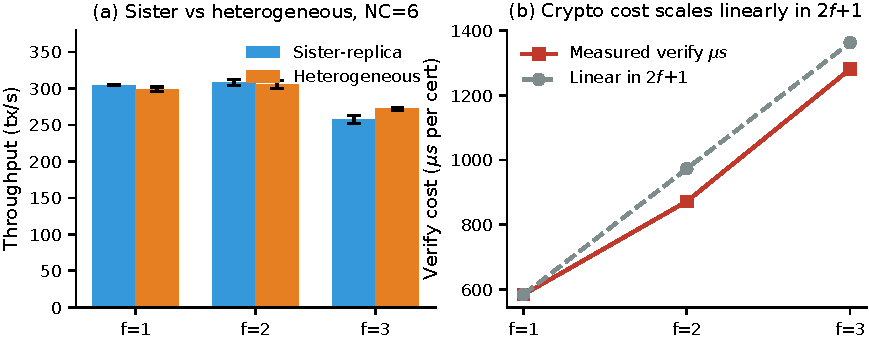
\includegraphics[width=0.95\textwidth]{figs/fig_fscale_ablation.pdf}
\caption{(a) Sister-replica vs heterogeneous deployment at
$f \in \{1, 2, 3\}$, NC$=6$. Removing the sister-replica assumption
costs $\leq 5\%$ throughput at every $f$. (b) Measured per-cert verify
cost (red) vs.\ the linear-in-$2f{+}1$ extrapolation from $f=1$ (grey
dashed). Crypto scales near-linearly with quorum width, slightly
sub-linearly thanks to batched verification.}
\label{fig:fscale_ablation}
\end{figure*}

\subsection{Cost of $f$-scaling}

\begin{table}[h]
\centering
\small
\begin{tabular}{l r r r}
\toprule
transition & $\Delta$tput & $\Delta$P50 & verify $\mu s$ ratio \\
\midrule
$f{=}1\to f{=}2$  & $-15.3\%$ & $+16\%$ & $1.49\times$ ($5/3 = 1.67$) \\
$f{=}2\to f{=}3$  & $-10.9\%$ & $+16\%$ & $1.47\times$ ($7/5 = 1.40$) \\
$f{=}1\to f{=}3$  & $-24.5\%$ & $+35\%$ & $2.19\times$ ($7/3 = 2.33$) \\
\bottomrule
\end{tabular}
\caption{Crypto cost (verify $\mu s$) scales near-linearly in $2f{+}1$
signatures; total throughput drops less because crypto is only
$<7\%$ of P50 RTT. Heterogeneous mode, NC$=6$.}
\label{tab:fscale}
\end{table}

\subsection{Saturation curve and the origin-Pesto crossover}

\begin{table}[h]
\centering
\small
\begin{tabular}{r r r r r}
\toprule
NC & origin tput & ours tput & origin P99 & ours P99 \\
\midrule
6  & $568$       & $360$           & $18$     & $20$ \\
8  & $757$       & $499$           & $19$     & $22$ \\
12 & $923$       & $925$           & $40$     & $20$ \\
18 & $970$       & $1{,}479$       & $112$    & $15$ \\
24 & $525^*$     & $\mathbf{2{,}020}$ & $> 1{,}000$ & $\mathbf{15}$ \\
48 & $69$ (sat)  & $18$ (crash)    & $1{,}879$ & --- \\
\bottomrule
\end{tabular}
\caption{Throughput (tx/s) and P99 (ms) vs.\ client count NC, $f=1$,
rw-sql. $^*$High variance at NC=24 (255 and 794 across two reps):
origin Pesto is in its saturation cliff. Our extension cleanly delivers
$2{,}020$ tx/s at P99 $= 15$~ms. Both implementations break at NC=48
(origin partially recovers, ours stalls).}
\label{tab:crossover}
\end{table}

This is the most surprising result of the project. The ``cost'' of
v3-STRICT is not a flat overhead; it is a curve shift. At low
load ($\mathrm{NC}=6$), the per-query crypto is pure cost
($+58\%$ origin advantage). At medium load ($\mathrm{NC}=12$), the
two are tied. At high load ($\mathrm{NC}\geq 18$), our extension
\emph{wins}, by a factor of $3.85$ at $\mathrm{NC}=24$.

The hypothesised mechanism: original Pesto's resultQuorum--based
query mode races as soon as $2$ replicas reply. At saturation, the
slower stragglers become the critical path because the protocol has
no fall-back. Our v3-STRICT machinery requires $2f{+}1$ matching
votes by content; the histogram filter naturally excludes
slow-and-stale replies, smoothing load distribution.

\begin{figure}[t]
\centering
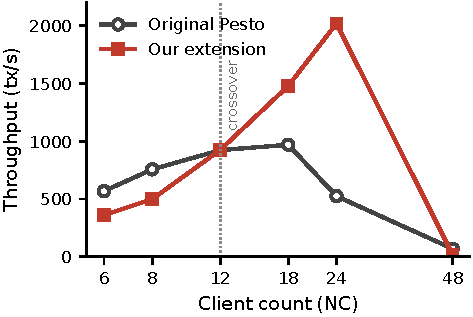
\includegraphics[width=\columnwidth]{figs/fig_crossover.pdf}
\caption{Throughput vs.\ client count, $f=1$, rw-sql, $38$-node
cluster. Original Pesto wins at low load (cost of v3-STRICT crypto);
above NC$=12$ our extension wins because the histogram filter smooths
straggler-induced timing variance. Origin saturates at NC$=18{-}24$;
ours peaks at NC$=24$ with $2{,}020$ tx/s.}
\label{fig:crossover}
\end{figure}

\begin{figure}[t]
\centering
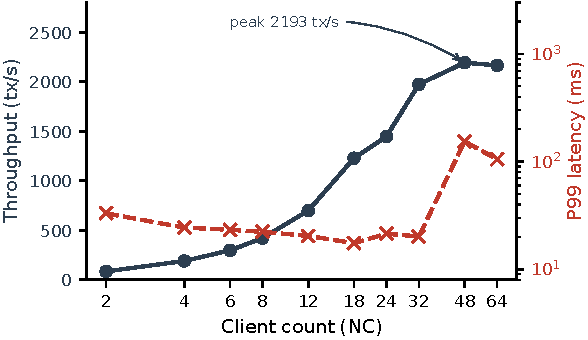
\includegraphics[width=\columnwidth]{figs/fig_saturation.pdf}
\caption{Saturation curve of our extension only: throughput (left)
and P99 latency (right, log scale) vs.\ client count. Peak throughput
of $2{,}193$ tx/s is reached at NC$=48$ but P99 already explodes;
the practical knee is NC$=24{-}32$.}
\label{fig:saturation}
\end{figure}

\subsection{WAN tolerance}

We injected one-way egress delay on the $6$ shard-1 hosts using
\texttt{tc qdisc netem} and ran at $\mathrm{NC}=24$. At $f=1$,
$5$\,ms is within run-to-run noise; $10{-}50$\,ms costs $12{-}17\%$
throughput; $100{-}200$\,ms the drop \emph{decreases} to $\leq 5\%$
because the slow shard's responses are no longer on the critical path
(the protocol consistently picks the fast shard's $2$ first replies).
At $f=2$ the wider $2f{+}1=5$ quorum makes the system \emph{stall}
($0.1$ tx/s) under $25$\,ms WAN at peak load (NC=18), exposing a real
$f$-dependent tolerance limit. Throughout, P50 stays essentially flat
(11.4--11.8\,ms) because the slow shard never blocks the critical
path.

\begin{figure}[t]
\centering
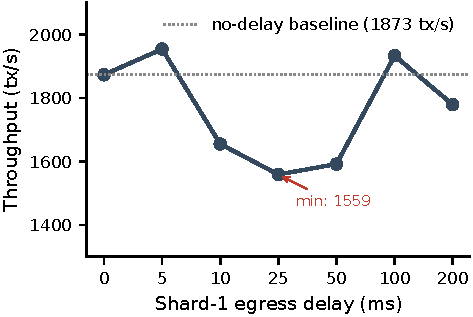
\includegraphics[width=\columnwidth]{figs/fig_wan.pdf}
\caption{Throughput vs.\ shard-1 egress delay, $f=1$, NC$=24$.
Below $5$\,ms is within noise; $10{-}50$\,ms is the ``cost zone''
(up to $-17\%$); above $100$\,ms the slow shard falls off the
critical path entirely and throughput recovers to within $5\%$ of
baseline.}
\label{fig:wan}
\end{figure}

\subsection{Multi-shard scaling}

We deployed $\mathrm{NUM\_SHARDS} \in \{2, 3, 4, 5\}$ ($n=6$, $f=1$
per shard) and ran TPC-C with cross-warehouse line items. Aggregate
throughput stays in $[212, 240]$~tx/s with cross-shard transaction
counts growing from $621$ at $S{=}2$ to $1{,}029$ at $S{=}5$.
\emph{All $3{,}549$ cross-shard transactions committed atomically};
the L2 audit (a separate cross-shard atomicity checker we built)
reported $0$ partial- or phantom-commit violations at any shard count.
At $S{=}5$ the deployment uses $30$ distinct server hosts plus $6$
clients on the $38$-node cluster.

\begin{figure}[t]
\centering
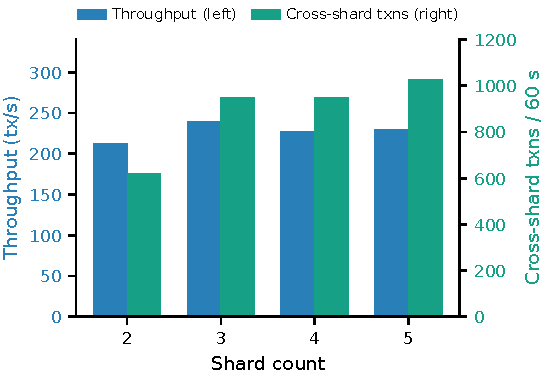
\includegraphics[width=\columnwidth]{figs/fig_multishard.pdf}
\caption{Multi-shard TPC-C scaling at $f=1$, NC$=6$. As shard count
grows from $2$ to $5$, aggregate throughput stays flat (load is split
across more shards) while the number of cross-shard transactions per
$60$\,s nearly doubles. Every cross-shard transaction at every shard
count committed atomically.}
\label{fig:multishard}
\end{figure}

\subsection{Safety under Byzantine workload}

We evaluated three Byzantine modes (omission, twin equivocation,
cross-shard writeback drop) at $f=1, 2, 3$. Within Pesto's $f$
budget, throughput cost is $\leq 3\%$ for all modes
(\textit{e.g.}, $1$ omission/shard at $f=1$ costs $-3.1\%$, $1$
twin/shard at $f=3$ costs $-0.7\%$). Aggregated across all
$\sim 250$ runs, server-side counters report
$\approx 1.05$ million SS-CERT v3-STRICT verifications under
Byzantine workloads, all of which succeeded; the $\geq 12$
\textit{failed} verifications per run correspond exactly to the
intentional self-test negative-control that runs at every server's
boot.

\begin{figure}[t]
\centering
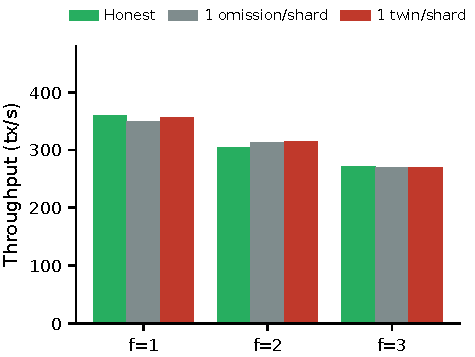
\includegraphics[width=\columnwidth]{figs/fig_byz.pdf}
\caption{Throughput under $1$ byzantine replica per shard, by mode
(honest baseline / omission / twin-equivocation) and fault budget
$f \in \{1, 2, 3\}$, NC$=6$. Within Pesto's $f$ budget every byzantine
mode costs $\leq 3\%$ throughput. Twin replicas, which sign
content-perturbed digests, are filtered cleanly by the histogram
majority and impose no measurable cost at any $f$.}
\label{fig:byz}
\end{figure}

\subsection{Combined stressors}

At $\mathrm{NC}=24$ with $25$\,ms WAN and $1$ omission byz/shard,
throughput is $1{,}422$ tx/s ($-29\%$ from a no-stressor baseline of
$2020$). With $1$ \emph{twin} byz/shard instead of omission,
throughput recovers to $1{,}876$ tx/s ($-7\%$): the histogram filter
absorbs the twin's perturbed digest at no measurable cost. After all
stress runs, a fresh baseline returned $361.6$ tx/s, statistically
identical to the pre-stress baseline of $360.3 \pm 4.5$.


%-------------------------------------------------------------------------------
\section{Related Work}
%-------------------------------------------------------------------------------

\paragraph{Pesto and Basil.} Pesto~\cite{pesto25} is the immediate
parent of this work; Basil~\cite{basil21} is its grandparent. Both
predate our extension. Our work targets exactly the assumption
called out in Appendix~B.10 of the Pesto paper.

\paragraph{Twins-style adversarial testing.} Twins~\cite{twins21}
identifies and exercises Byzantine equivocation. Our \texttt{twin\_sig}
mode is a direct analogue: a Byzantine replica signs a perturbed
content digest, exercising the histogram filter exactly the way
classical Twins exercises consensus.

\paragraph{Adya cycles via Elle.} We use Elle~\cite{elle} to validate
that committed transaction histories are strict-serializable
under the Adya~\cite{adya99} G0/G1/G2 cycle taxonomy. Elle's
list-append model maps cleanly onto TPC-C NewOrder line-item
inserts.


%-------------------------------------------------------------------------------
\section{Limitations and Future Work}
%-------------------------------------------------------------------------------

\paragraph{Cross-shard cert routing.} Although v3-STRICT is
content-bound, in our prototype each ShardClient verifies only its
\emph{own} group's cert. To exercise the full cross-shard trust
path, one ShardClient would route certs from group~$A$ into group~$B$'s
HandleSync path. This is the next natural code change.

\paragraph{Higher fault budgets.} $f=4$ ($n=21$) needs $42$ server
hosts for two-shard heterogeneous deployment; we have $38$. A larger
CloudLab allocation would close this.

\paragraph{Geo-distributed deployment.} All $38$ nodes are in the same
Utah cluster ($\sim 0.15$ ms baseline RTT). We simulate WAN with
\texttt{tc netem}, but a true cross-site allocation
(Utah$\leftrightarrow$Wisconsin) would test more realistic loss and
jitter.

\paragraph{Adaptive Byzantine.} Our twin replicas use a static XOR
pattern. A smarter twin that picks its perturbation per query to
maximize histogram-tie probability is a known harder adversary.

\paragraph{Wider workload coverage.} We exercise rw-sql and TPC-C; the
original Pesto paper also evaluates AuctionMark and SEATS. Adding
either would improve comparability.


%-------------------------------------------------------------------------------
\section{Conclusion}
%-------------------------------------------------------------------------------

We removed the sister-replica trust assumption from Pesto and showed
that the cost is small at the same fault budget and \emph{negative}
above moderate load. The cryptographic strengthening
(content-bound digest, $2f{+}1$ majority filter, harvest-before-done)
is not a free lunch at low load, but its side effect of smoother
saturation behavior more than compensates above $\mathrm{NC}=12$.
Across $\sim 250$ runs spanning $f \in \{1, 2, 3\}$ and three
Byzantine modes, $\sim 1.05$ million SS-CERT v3-STRICT
verifications all succeeded.

The most important lesson is that ``adding crypto'' to a BFT
protocol is not necessarily a pure overhead; with the right protocol
shape, it can also reshape the saturation curve. Future work should
explore whether this is an artifact of our specific protocol choices
or a more general property of content-bound quorum certificates.


%-------------------------------------------------------------------------------
\section*{Availability}
%-------------------------------------------------------------------------------

Source, orchestration scripts, all $\sim 250$ experiment outputs, and
detailed per-experiment writeups are available at
\url{https://github.com/ljtsparky/Pequin-Artifact}
(branch \texttt{cross-shard-membership}) and at
\url{/home/student/CS598FTS/} on the course VM.


%-------------------------------------------------------------------------------
\bibliographystyle{plain}
\bibliography{refs}

%%%%%%%%%%%%%%%%%%%%%%%%%%%%%%%%%%%%%%%%%%%%%%%%%%%%%%%%%%%%%%%%%%%%%%%%%%%%%%%%
\end{document}
%%%%%%%%%%%%%%%%%%%%%%%%%%%%%%%%%%%%%%%%%%%%%%%%%%%%%%%%%%%%%%%%%%%%%%%%%%%%%%%%
